\chapter{Evaluation}

With the setup explained in Section~\ref{imp.ch}, we will now compile, evaluate with QEMU, and flash the binaries onto our boards.

\section{Compilation} \label{comp.ch}
\subsection{Sample Code}

\begin{figure}[H]
\centering
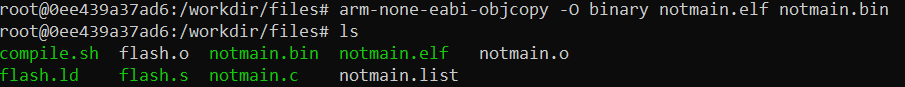
\includegraphics[width=0.8\textwidth]{samplecompdir.png}
\caption{Sample code directory after compilation}
\label{fig:samplecomp}
\end{figure}

To compile this sample code for the target platform the commands shown in Listing~\ref{compSample} are issued through the command line shell \code{bash}. Initially starting with three files \code{flash.s}, \code{notmain.c} and \code{flash.ld}, we are now presented with five additional files. \code{flash.o}, \code{notmain.o}, \code{notmain.elf}, \code{notmain.list} and most importantly \code{notmain.bin}, the "sample kernel", as seen in Figure~\ref{fig:samplecomp}. From Listing~\ref{compSample} we can also see the flag \code{-mcpu=cortex-m4}, symbolizing that we are compiling for target platform ARM Cortex-M4.

\begin{lstlisting}[style=SH, caption=Compiling sample code with gcc-arm-none-eabi toolchain, label=compSample, float, floatplacement=H]
arm-none-eabi-as -warn -fatal-warnings \
-mcpu=cortex-m4 flash.s -o flash.o
arm-none-eabi-gcc -Wall -O2 -ffreestanding \
-mcpu=cortex-m4 -mthumb -c notmain.c -o notmain.o
arm-none-eabi-ld -nostdlib -nostartfiles -T flash.ld flash.o notmain.o \
-o notmain.elf
arm-none-eabi-objdump -D notmain.elf > notmain.list
arm-none-eabi-objcopy -O binary notmain.elf notmain.bin
\end{lstlisting}

\subsection{U-Boot}

\begin{figure}[H]
\centering
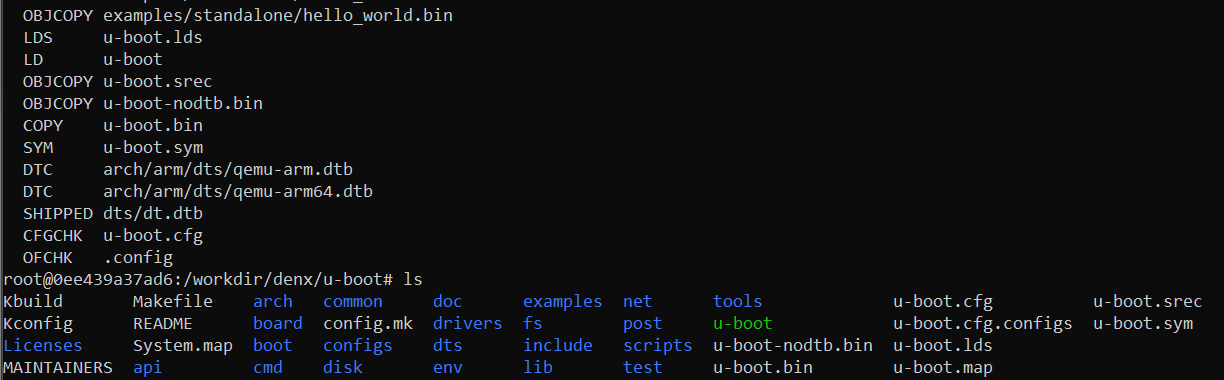
\includegraphics[width=0.8\textwidth]{u-bootqemucomp.png}
\caption{Executing Listing~\ref{compQEMUuboot} with output files}
\label{fig:u-bootqemucomp}
\end{figure}

As a first step, we will compile U-Boot for QEMU, so that we can continue evaluating, without needing to flash onto an MCU every time. If not previously done so, we need to navigate inside the folder. Using our previously established toolchain, \code{gcc-arm-none-eabi}, we call the commands, shown in Listing~\ref{compQEMUuboot} inside of the current folder. At line 2 of Listing~\ref{compQEMUuboot}, \code{qemu\_arm\_defconfig}, is mentioned after having declared the toolchain. This config is simply a pre-set configuration file that is provided by U-Boot, for specific targets. After compilation is completed, taking about 30 seconds, \code{u-boot.bin} is the main output of our compilation, as seen in Figure~\ref{fig:u-bootqemucomp}.

\begin{lstlisting}[style=SH, caption=Compiling U-Boot for QEMU, label=compQEMUuboot]
make mrproper
make ARCH=arm CROSS_COMPILE=arm-none-eabi- qemu_arm_defconfig
make ARCH=arm CROSS_COMPILE=arm-none-eabi-
\end{lstlisting}



\subsection{Mainline Linux kernel}
A similar approach is taken within the directory of the Linux kernel source code. Firstly we make sure that previous configurations and compilations are deleted, this is achieved with line 1 in Listing~\ref{lst:complinux} \code{make mrproper}. On line 2 we set the \code{stm32\_defconfig} as our config since we are trying to compile Linux for STM32 systems.

\begin{lstlisting}[style=SH, caption=Compiling the Linux kernel, label=lst:complinux]
make ARCH=arm CROSS_COMPILE=arm-none-eabi- mrproper
make ARCH=arm stm32_defconfig
make ARCH=arm CROSS_COMPILE=arm-none-eabi- xipImage
make ARCH=arm CROSS_COMPILE=arm-none-eabi- dtbs
\end{lstlisting}

\begin{figure}[H]
\centering
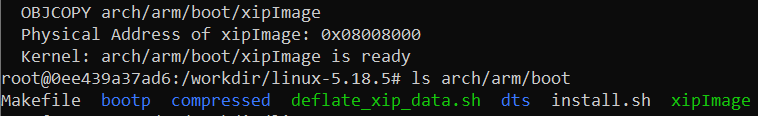
\includegraphics[width=0.8\textwidth]{mainlineLinuxComp.png}
\caption{Directory after Linux compilation of Listing~\ref{lst:complinux}}
\label{fig:buildroot-menuconfig}
\end{figure}

After line 3 of Listing~\ref{lst:complinux} we succesfully compiled \code{xipImage} which is located in \code{./arch/arm/boot}.

\begin{figure}[H]
\centering
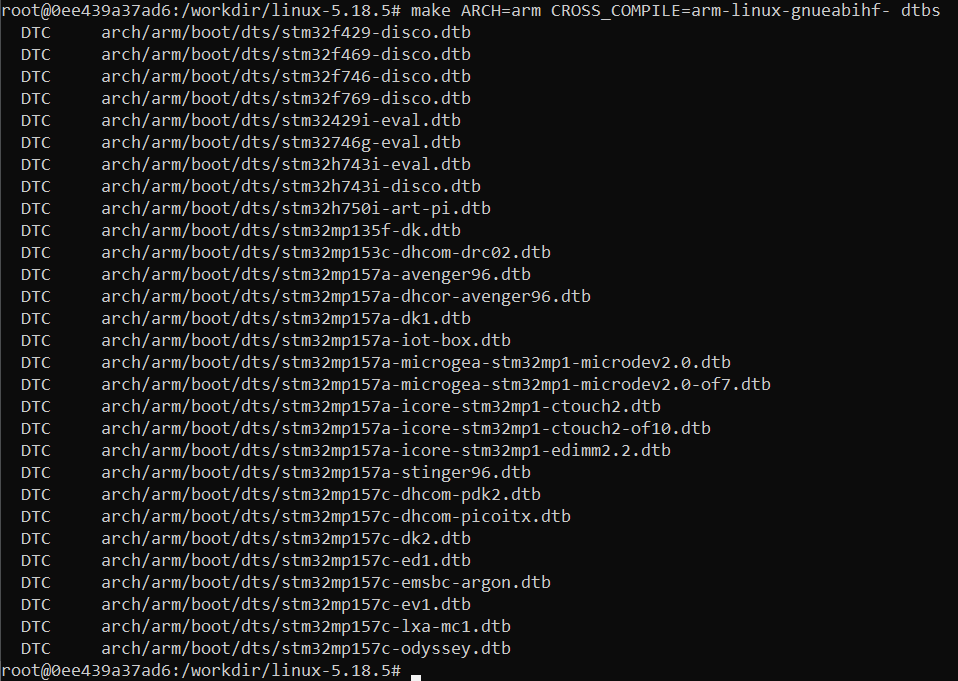
\includegraphics[width=0.8\textwidth]{dtbslinuxcomp.png}
\caption{Output after running line 4 of Listing \ref{lst:complinux}}
\label{fig:linuxcompdtb}
\end{figure}

In Figure~\ref{fig:linuxcompdtb} we can see all the device trees that are created upon the conclusion of line 4 of Listing \ref{lst:complinux}. Unfortunately, our board, seen in Figure~\ref{stm32l}, is not present.

\begin{figure}[H]
\centering
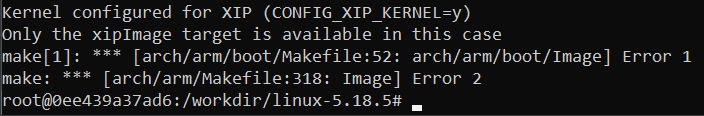
\includegraphics[width=0.8\textwidth]{linuxcompzimageerror.png}
\caption{Error: using \code{zImage} as output instead of \code{xipImage} in Listing \ref{lst:complinux}}
\label{fig:errorlinuxcompzimage}
\end{figure}

In the error shown in Figure \ref{fig:errorlinuxcompzimage}, we can see that if choosing the wrong output for our compilation, or a different output than the one defined in our \code{.config} file, we get an error. 

\subsection{$\mu$Clinux}
A similar approach is taken for $\mu$Clinux. Unter \code{arch/arm/configs}, we find the different configurations, the closest to our current board are \code{stm32f2\_defconfig}, \code{stmp378x\_defconfig} and \code{stmp37xx\_defconfig}. The ones labled with \code{stmp} are refering to boards with MPUs, as described in section~\ref{mcuvsmpu.ch}. 


\begin{lstlisting}[style=SH, caption=Compiling $\mu$Clinux, label=lst:compuclinux]
make stm32f2_defconfig
make CROSS_COMPILE=arm-uclinuxeabi- vmlinux
\end{lstlisting}

To prove that the toolchains and the setup work we can start compilation with commands shown in Listing~\ref{lst:compuclinux}. During the compilation process \code{warning}'s are shown, this could be due to the age of this $\mu$Clinux distribution, yet it completes successfully. The output is a \code{vmlinux} file.


\subsection{Buildroot} \label{compbuildroot.ch}
We have to navigate to the Buildroot directory. In the documentation of Buildroot, under 2.1. "Mandatory packages", a list of required dependencies for the compilation process are shown, we have installed some of these packages in Section~\ref{envsetup.ch}, and others come with the Ubuntu 20.04 LTS distribution. Equivalently to the previous steps, the \code{configs} directory holds all the pre-set configuration files that can be used to compile Linux, by navigating to the directory we see all the configs that can be used, and later on modified. Unfortunately STM32L476G-Eval is not included, but other configurations for STM are available, such as \code{stm32f429\_disco\_sd\_defconfig} for the STM32F429-Discovery development board. \code{make stm32f469\_disco\_sd\_defconfig} will copy the code from the specified configuration into the \code{.config} file, which is not visible in the thee unless command \code{ls -a} is issued.

\begin{lstlisting}[style=SH, caption=buildroot, label=buildroot]
make stm32f469_disco_sd_defconfig
make
\end{lstlisting}

\begin{figure}[H]
\centering
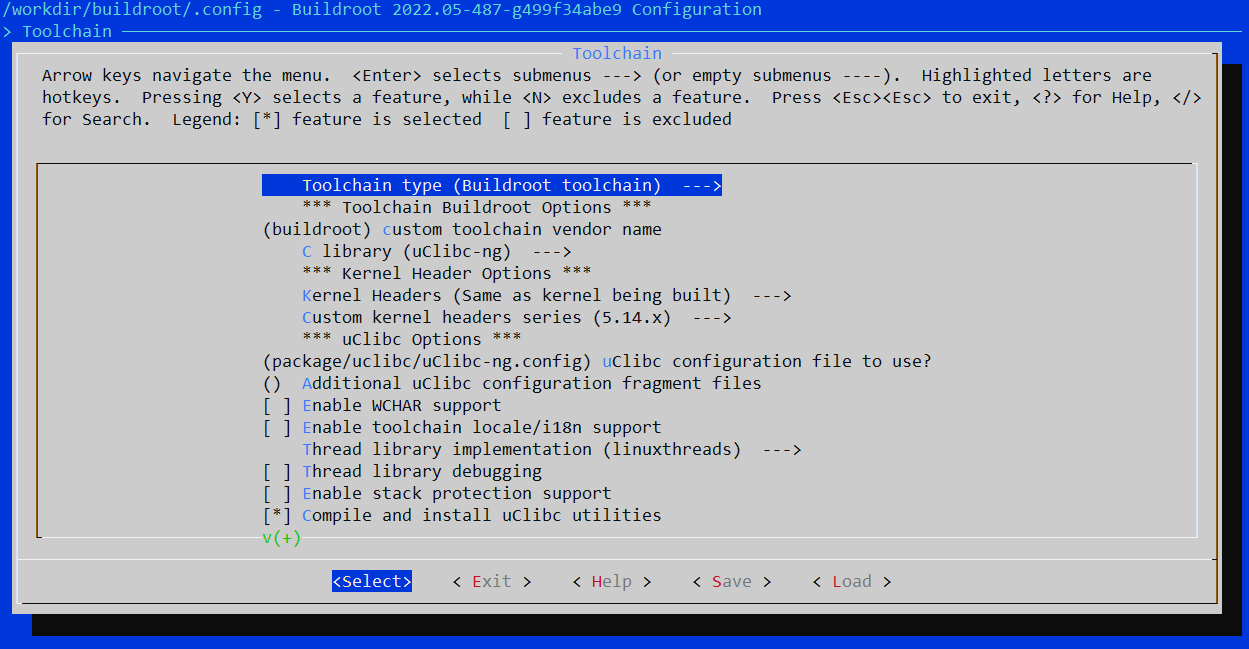
\includegraphics[width=0.8\textwidth]{buildrootmenuconfigtoolchain.png}
\caption{Buildroot \code{make menuconfig} / Toolchain}
\label{buildrootmenuconfigtoolchain}
\end{figure}

To get further insight into what the Buildroot configuration has specified we can type command \code{make menuconfig} inside the directory, we are loaded into the visual configuration menu displayed in the console that can help us visually navigate through the \code{.config} file and configure our build further. Note that for this visual editor the \code{libncurses5-dev} package is required and was installed in section \ref{envsetup.ch}. This is shown in Figure \ref{buildrootmenuconfigtoolchain}. An interesting variation is to be observed, the library mentioned in section \ref{uclinux.ch}, \code{uClibc-ng}, is used.

With \code{make}, the compilation process starts. Depending on the local machine that is performing the process, this process can be very time and resource-intensive. Once complete, the outputs will appear in a new folder inside the Buildroot directory under \code{output}, the contents are shown in Figure~\ref{buildrootoutput}. \code{u-boot.bin} and \code{rootfs.ext2} were created automatically, \code{sdcard.img} can be flashed directly onto out SD-card. The usual \code{zImage} and device tree \code{stm32f469-disco.dtb} are also present. While compilation here required much more time than any of the previous compilations, Buildroot shows much promise because we are not required to configure and compile any other tools.

\begin{figure}[H]
\centering
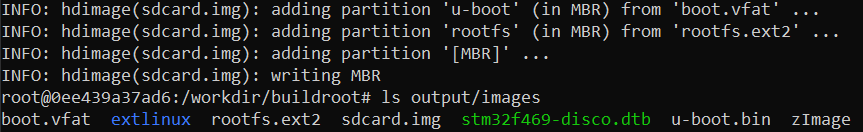
\includegraphics[width=0.8\textwidth]{buildrootoutput.png}
\caption{The \code{output/images} directory after Buildroot compilation}
\label{buildrootoutput}
\end{figure}

\begin{lstlisting}[style=SH, caption=Compiling commands used in Buildroot directory, label=compbuildroot]
make stm32f469_disco_sd_defconfig
make
\end{lstlisting}

\begin{figure}[H]
\centering
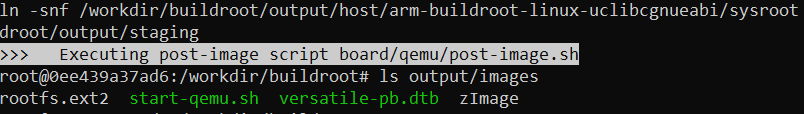
\includegraphics[width=0.8\textwidth]{buildrootoutputqemu.png}
\caption{The \code{output/images} directory for QEMU}
\label{buildrootoutputqemu}
\end{figure}

Equivalently to Listing~0\ref{compbuildroot}, we can use \code{make qemu\_arm\_versatile\_defconfig} instead of line 1 to compile a linux distribution specifically for QEMU. With this \code{defconfig} the output is shown in Figure \ref{buildrootoutputqemu}. Most notably the \code{start-qemu.sh} script.


\section{Emulating with QEMU}
After having compiled the various source code in Section~\ref{comp.ch}, the next step is to emulate using QEMU. To leave QEMU press CTRL+A and X.

\subsection{Sample Code}

\begin{figure}[H]
\centering
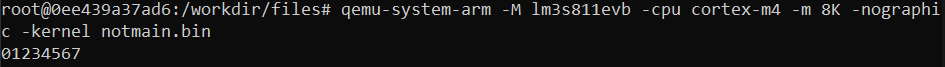
\includegraphics[width=0.9\textwidth]{sampleqemu.png}
\caption{Executing Listing \ref{sampleqemu}}
\label{fig:sampleqemu}
\end{figure}

Although in QEMUs documentation~\cite{qemuarm} it is stated that \code{netduinoplus2}, \code{netduino2} and \code{stm32vldiscovery} are supported and are the closest to our board, only \code{netduino2} is actually available. If we run qemu with this machine, flagged as the \code{-M netduino2}, we do not get an output. When using commands from Listing~\ref{sampleqemu} we get the desired output seen in Figure~\ref{fig:sampleqemu}.

\begin{lstlisting}[style=SH, caption=Running sample code with QEMU, label=sampleqemu]
qemu-system-arm -M lm3s811evb -cpu cortex-m4 \
 -m 8K -nographic -kernel notmain.bin
\end{lstlisting}

\subsection{U-Boot}
\begin{figure}[H]
\centering
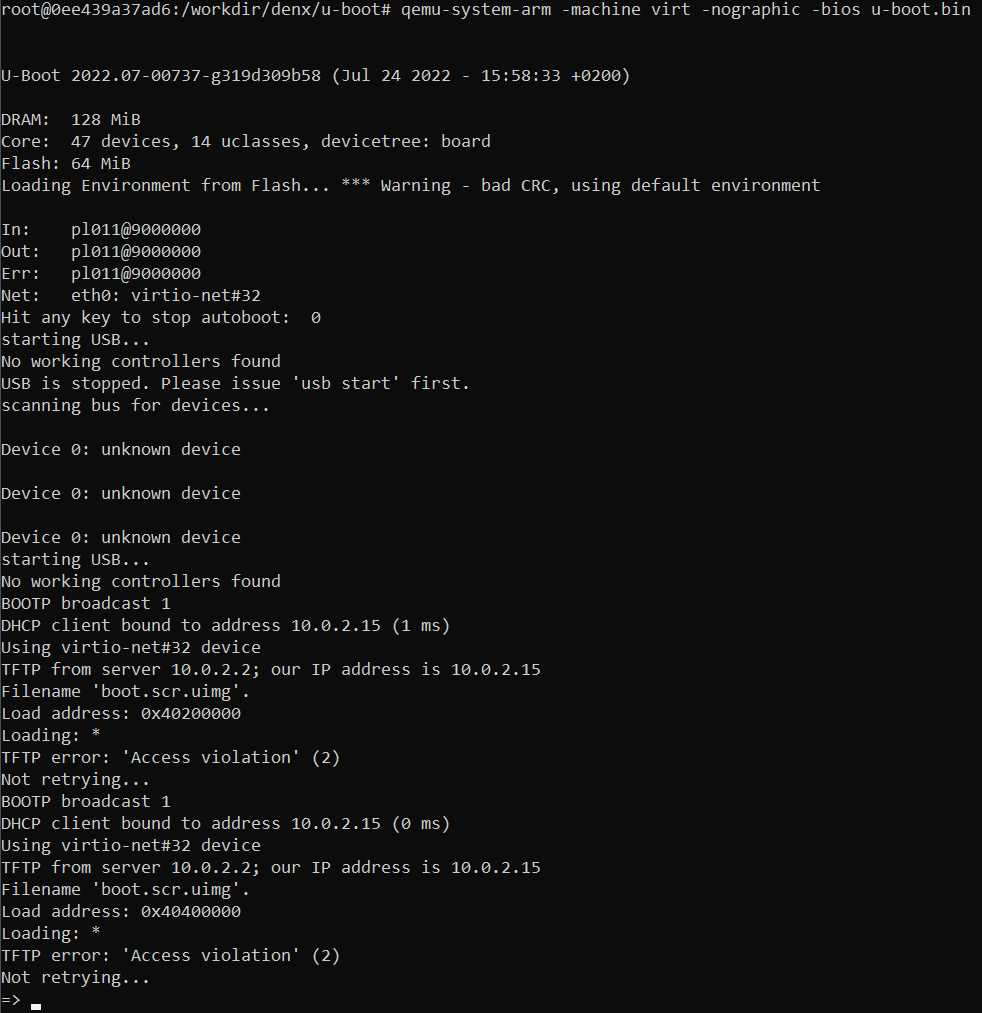
\includegraphics[width=0.8\textwidth]{ubootqemu.png}
\caption{Running U-boot with QEMU}
\label{ubootqemu}
\end{figure}

By running the command seen in Listing~\ref{runQEMUuboot}, we successfully loaded the bootloader with QEMU, as shown in Figure~\ref{ubootqemu}. We are presented with the CLI of U-boot.

\begin{lstlisting}[style=SH, caption=Running U-Boot with QEMU, label=runQEMUuboot]
qemu-system-arm -machine virt -nographic -bios u-boot.bin
\end{lstlisting}

\subsection{Buildroot} \label{success}
\begin{figure}[H]
\centering
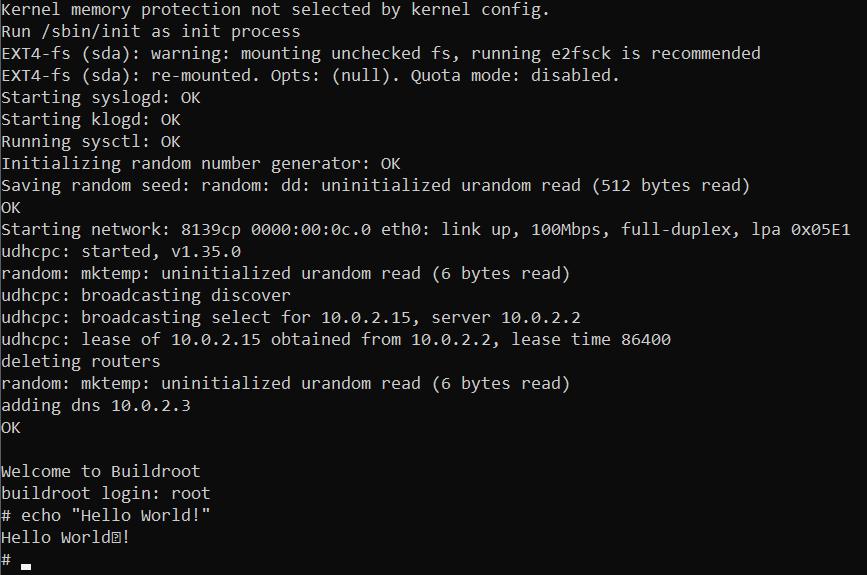
\includegraphics[width=0.8\textwidth]{buildrootqemu.png}
\caption{Starting Buildroot Linux with QEMU}
\label{buildrootqemu}
\end{figure}

Seen in Figure~\ref{buildrootqemu}, by activating the \code{start-qemu.sh} script previously compiled in Section~\ref{compbuildroot.ch} a prompt ask us to provide login credentials, upon entering \code{root}, the system grants us access and we are loaded in Linux's typical \code{sh} shell. This exhausts the requirements of this thesis, as it provides a Linux distribution running on MCUs, emulated with QEMU.

\begin{figure}[H]
\centering
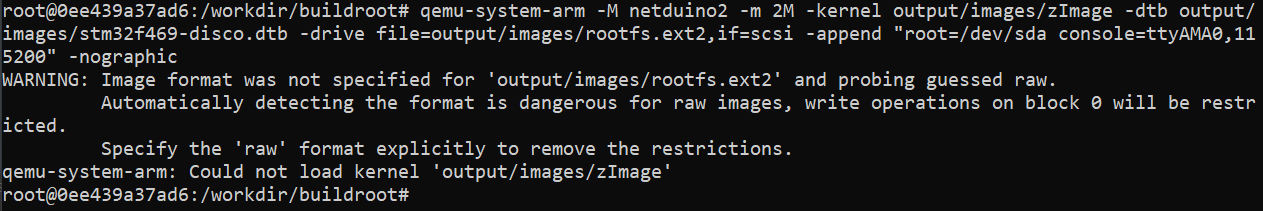
\includegraphics[width=0.9\textwidth]{buildrootQEMUstm.png}
\caption{Error: Starting Buildroot \code{stm32f469\_disco\_sd\_defconfig} configuration}
\label{fig:buildrootqemustm}
\end{figure}

Alternatively trying to start the distribution compiled with the \code{stm32f469\_disco\_sd\_defconfig} configuration, compiled in Section~\ref{compbuildroot.ch}, when running the command seen in Listing~\ref{runQEMUbuildroot} in the Buildroot directory, the kernel could not be loaded. The results are shown in Figure~\ref{fig:buildrootqemustm}. Because we do not have the exact board.

\begin{lstlisting}[style=SH, caption=Running Buildroot Linux with QEMU, label=runQEMUbuildroot]
qemu-system-arm -M netduino2 \
-kernel output/images/zImage \
-dtb output/images/stm32f469-disco.dtb \
-drive file=output/images/rootfs.ext2,if=scsi \
-append "root=/dev/sda console=ttyAMA0,115200" \
-nographic
\end{lstlisting}

\section{Flashing binaries} \label{flashing.ch}
In this Section, we are flashing compiled binaries onto our devices and SD card, namely STM32L476G-Eval~\ref{stm32l} and ESP-EYE DevKit~\ref{esp-eye}.

\subsection{FreeRTOS on STM32L4}

\begin{figure}[H]
\centering
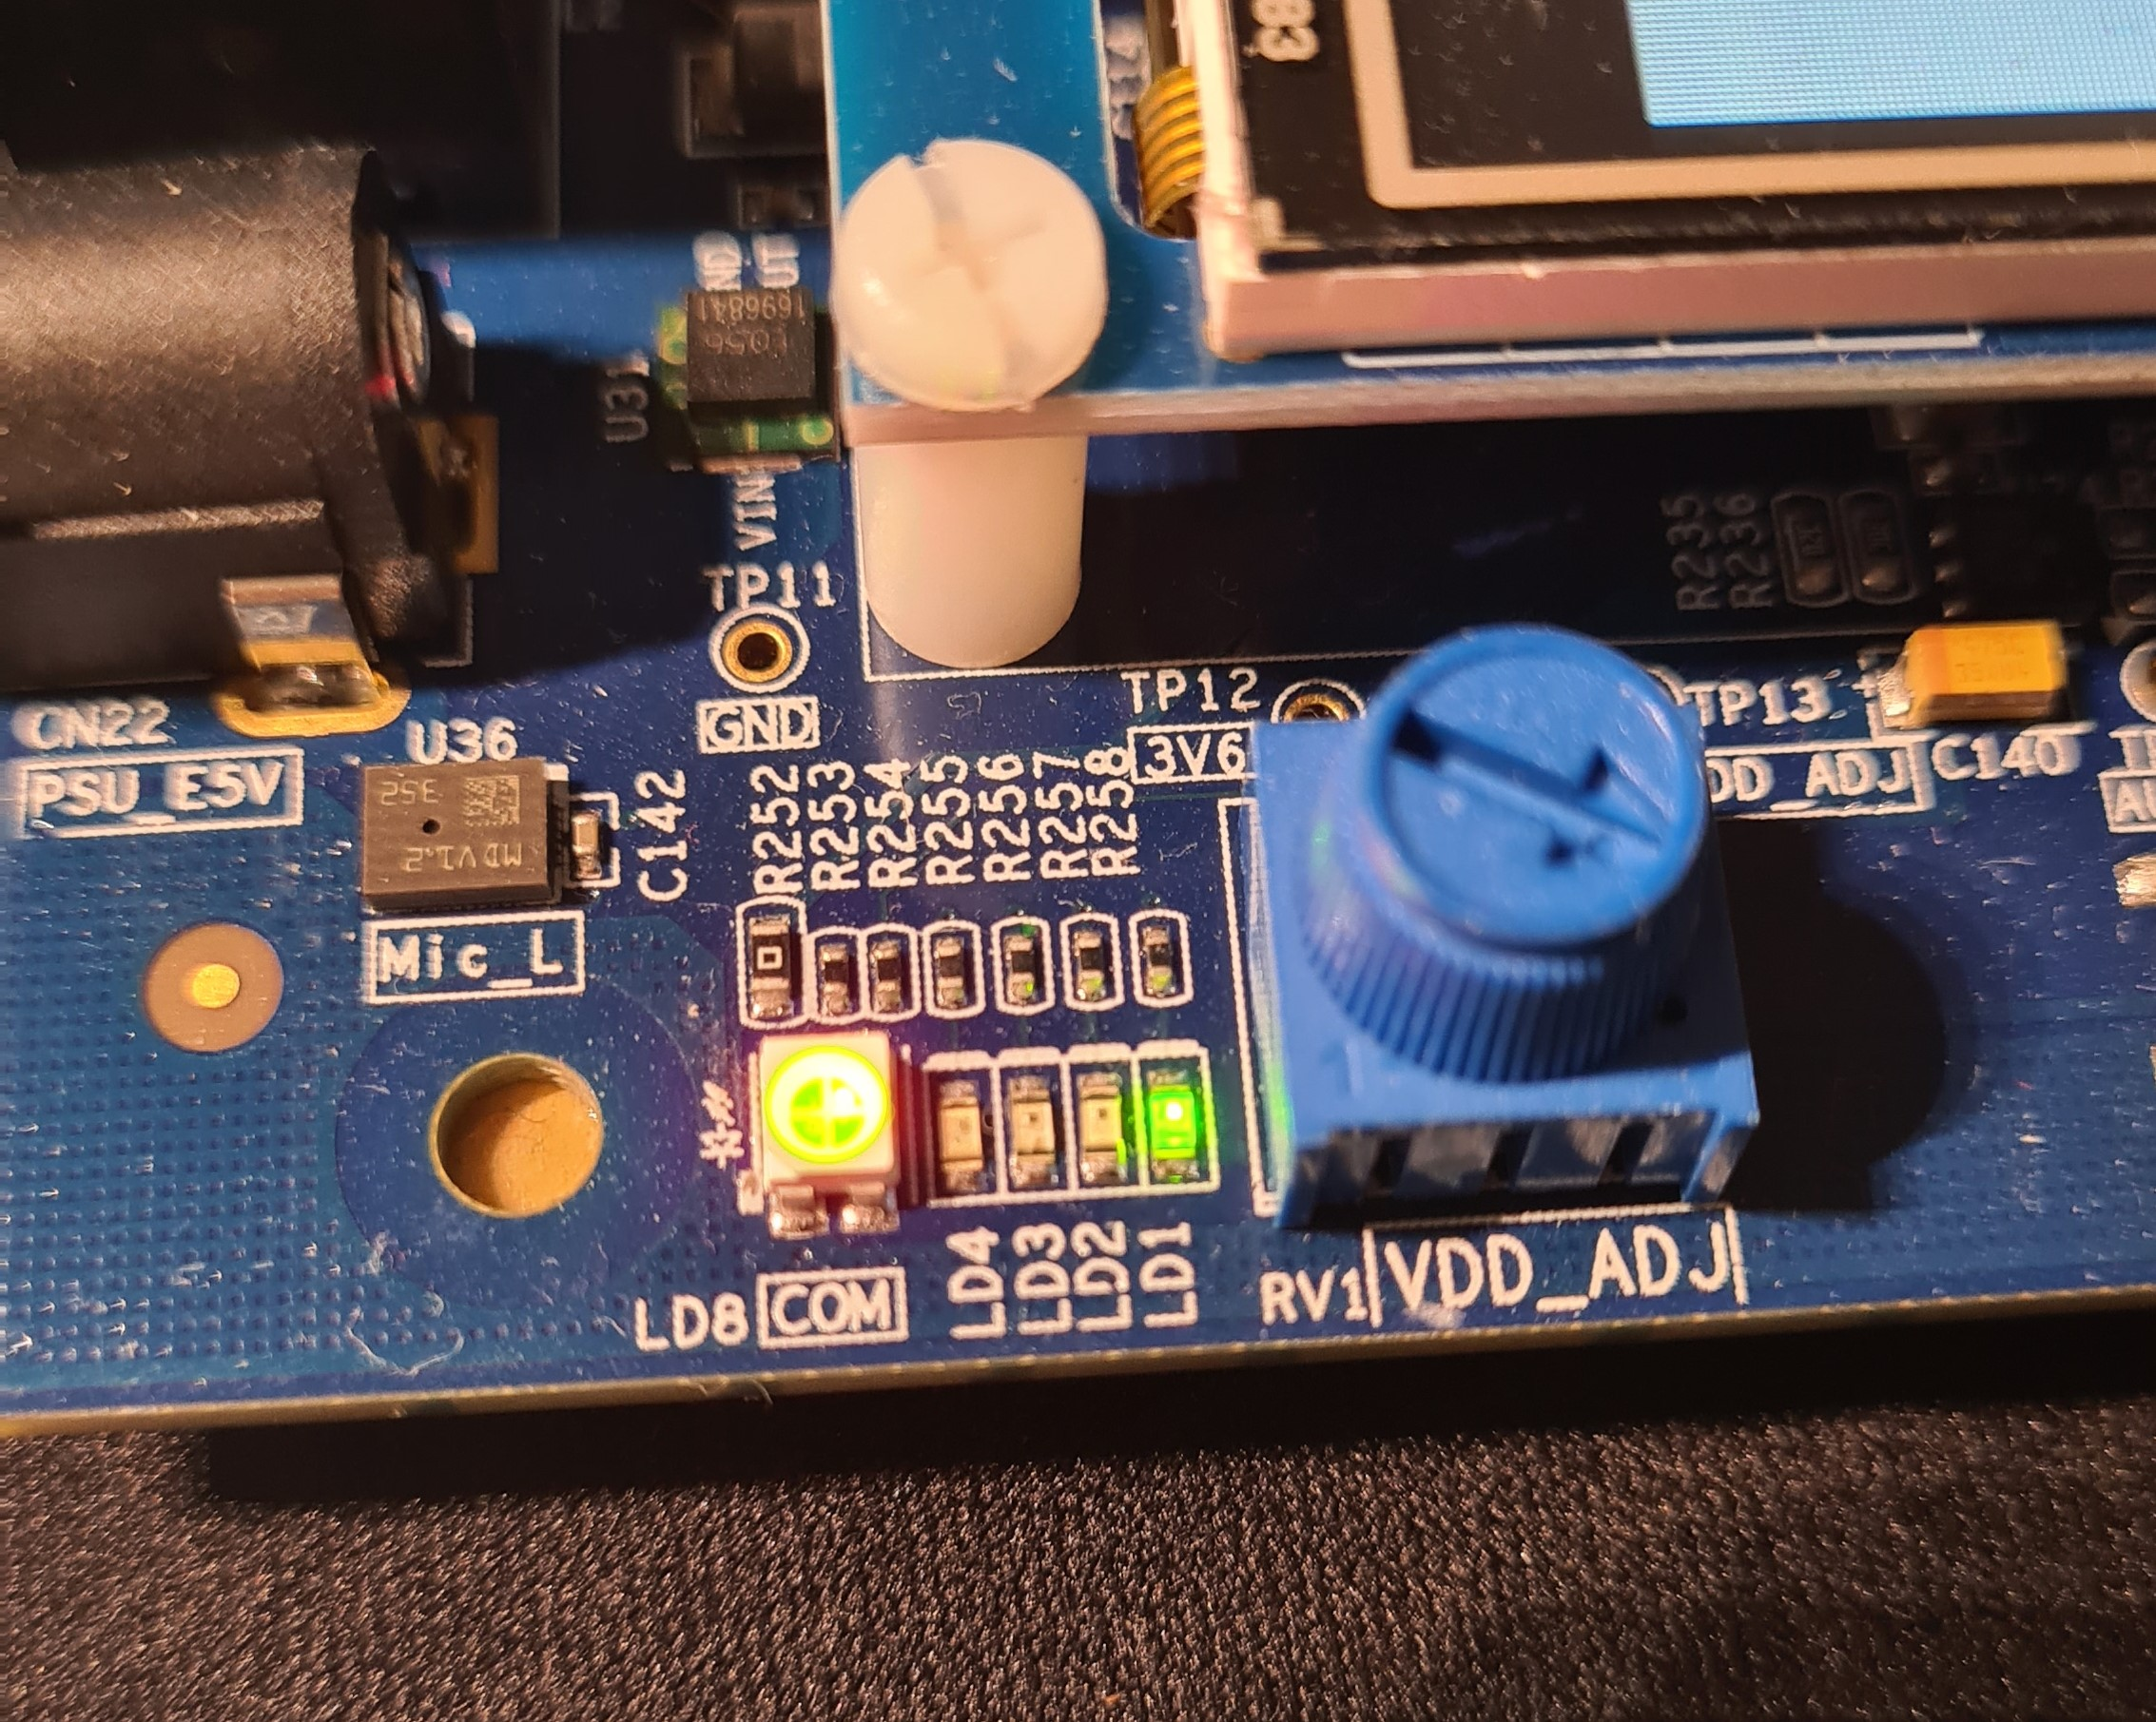
\includegraphics[width=0.6\textwidth]{BlinkingLD1.jpg}
\caption{Blinking \code{LD1}}
\label{fig:blinking}
\end{figure}

Since STM32CubeIDE was used, which includes the required toolchains and libraries, the compilation process is facilitated and was not worth mentioning in the previous chapter. By running the compiled binaries as an "STM32 Cortex-M C/C++ Application" we can observe that the system behaves correctly, and the \code{LD1} flashes in a periodic manner described best by the \code{sin()} function. As the two threads compete to toggle the LD, with different \code{osDelay}s, 600 and 500, respectively. In Figure~\ref{fig:blinking}, we can see that the light is on, as blinking is hard to capture in a picture.

\subsection{JuiceVM}

\begin{lstlisting}[style=SH, caption=Flashing JuiceVM to ESP-EYE, label=flashJuiceVM]
.\esptool.exe -chip esp32 -port COM7 erase_flash
.\esptool.exe -chip esp32 -port COM7 ^
-baud 460800 write_flash -z 0x1000 ^
.\juicevm-risc-v_vm-for-esp32_wrover-linux_demo.bin
\end{lstlisting}

To flash the binaries provided by JuiceVM, namely the \code{juicevm-risc-v\_vm-for-esp32\_wrover-linux\_demo.bin}, onto the ESP-EYE DevKit, we require the previously mentioned \code{esptool.exe}. By executing commands seen in Listing~\ref{flashJuiceVM} inside the directory where the binary file is located. Note that this command was executed on the host OS, which in this case was Windows 10.

\begin{figure}[H]
\centering
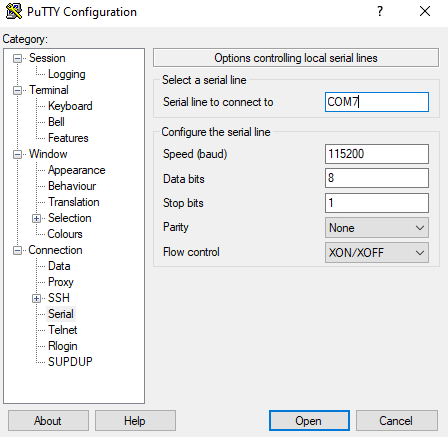
\includegraphics[width=0.6\textwidth]{puttyjuiceVM.png}
\caption{PuTTY configuration to connect to display JuiceVMs console}
\label{puttyjuiceVM}
\end{figure}

After flashing has been completed a connection to the console through the serial console using PuTTY is possible. It was not possible to connect to the serial port beforehand because it was occupied with flashing the files. To achieve this baud rate is set to 115200, data bits to 8, stop bits to 1, party to none, and flow control to XON/XOFF, this is shown in Figure \ref{puttyjuiceVM}. If a wrong baud rate is chosen, for example, the one specified in Listing~\ref{flashJuiceVM}, an output is visible but not coherent.

\begin{figure}[H]
\centering
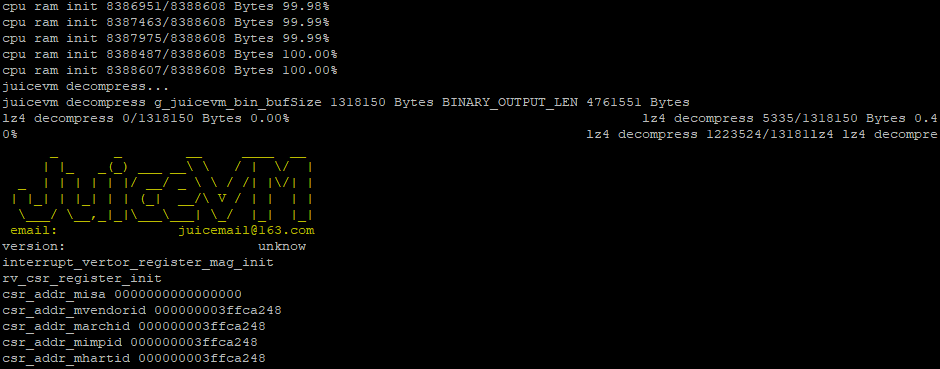
\includegraphics[width=0.8\textwidth]{juiceVMlogo.png}
\caption{PuTTY: JuiceVM console after more than 10 hours}
\label{juiceVMlogo}
\end{figure}

JuiceVM commences by initializing CPU RAM, up to about 99\% this process is completed very rapidly, after which it slows down significantly. Upon completion, decompression is next, which after nearly 10 hours, only reached 92\%. Figure~\ref{juiceVMlogo}, shows CPU RAM initialization, decompression, and a loaded JuiceVM.

\begin{figure}[H]
\centering
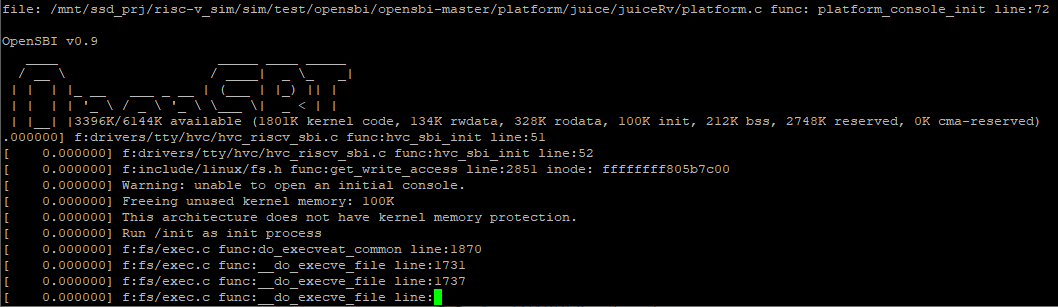
\includegraphics[width=0.8\textwidth]{juiceVM32h.png}
\caption{PuTTY: JuiceVM console after 32 hours}
\label{juiceVM32h}
\end{figure}

After close to 32 hours, seen in Figure~\ref{juiceVM32h}, it was decided to quit the proceedings due to the unusably long boot process. At this point the \code{printk()} function took 12 seconds to print a character to the console. Interestingly we can see the line \code{Freeing unused kernel memory: 100K}, which was making space in the main memory for other objects. The reason for such a long boot process is not known, and requires further investigation. 

\subsection{Buildroot}

\begin{figure}[H]
\centering
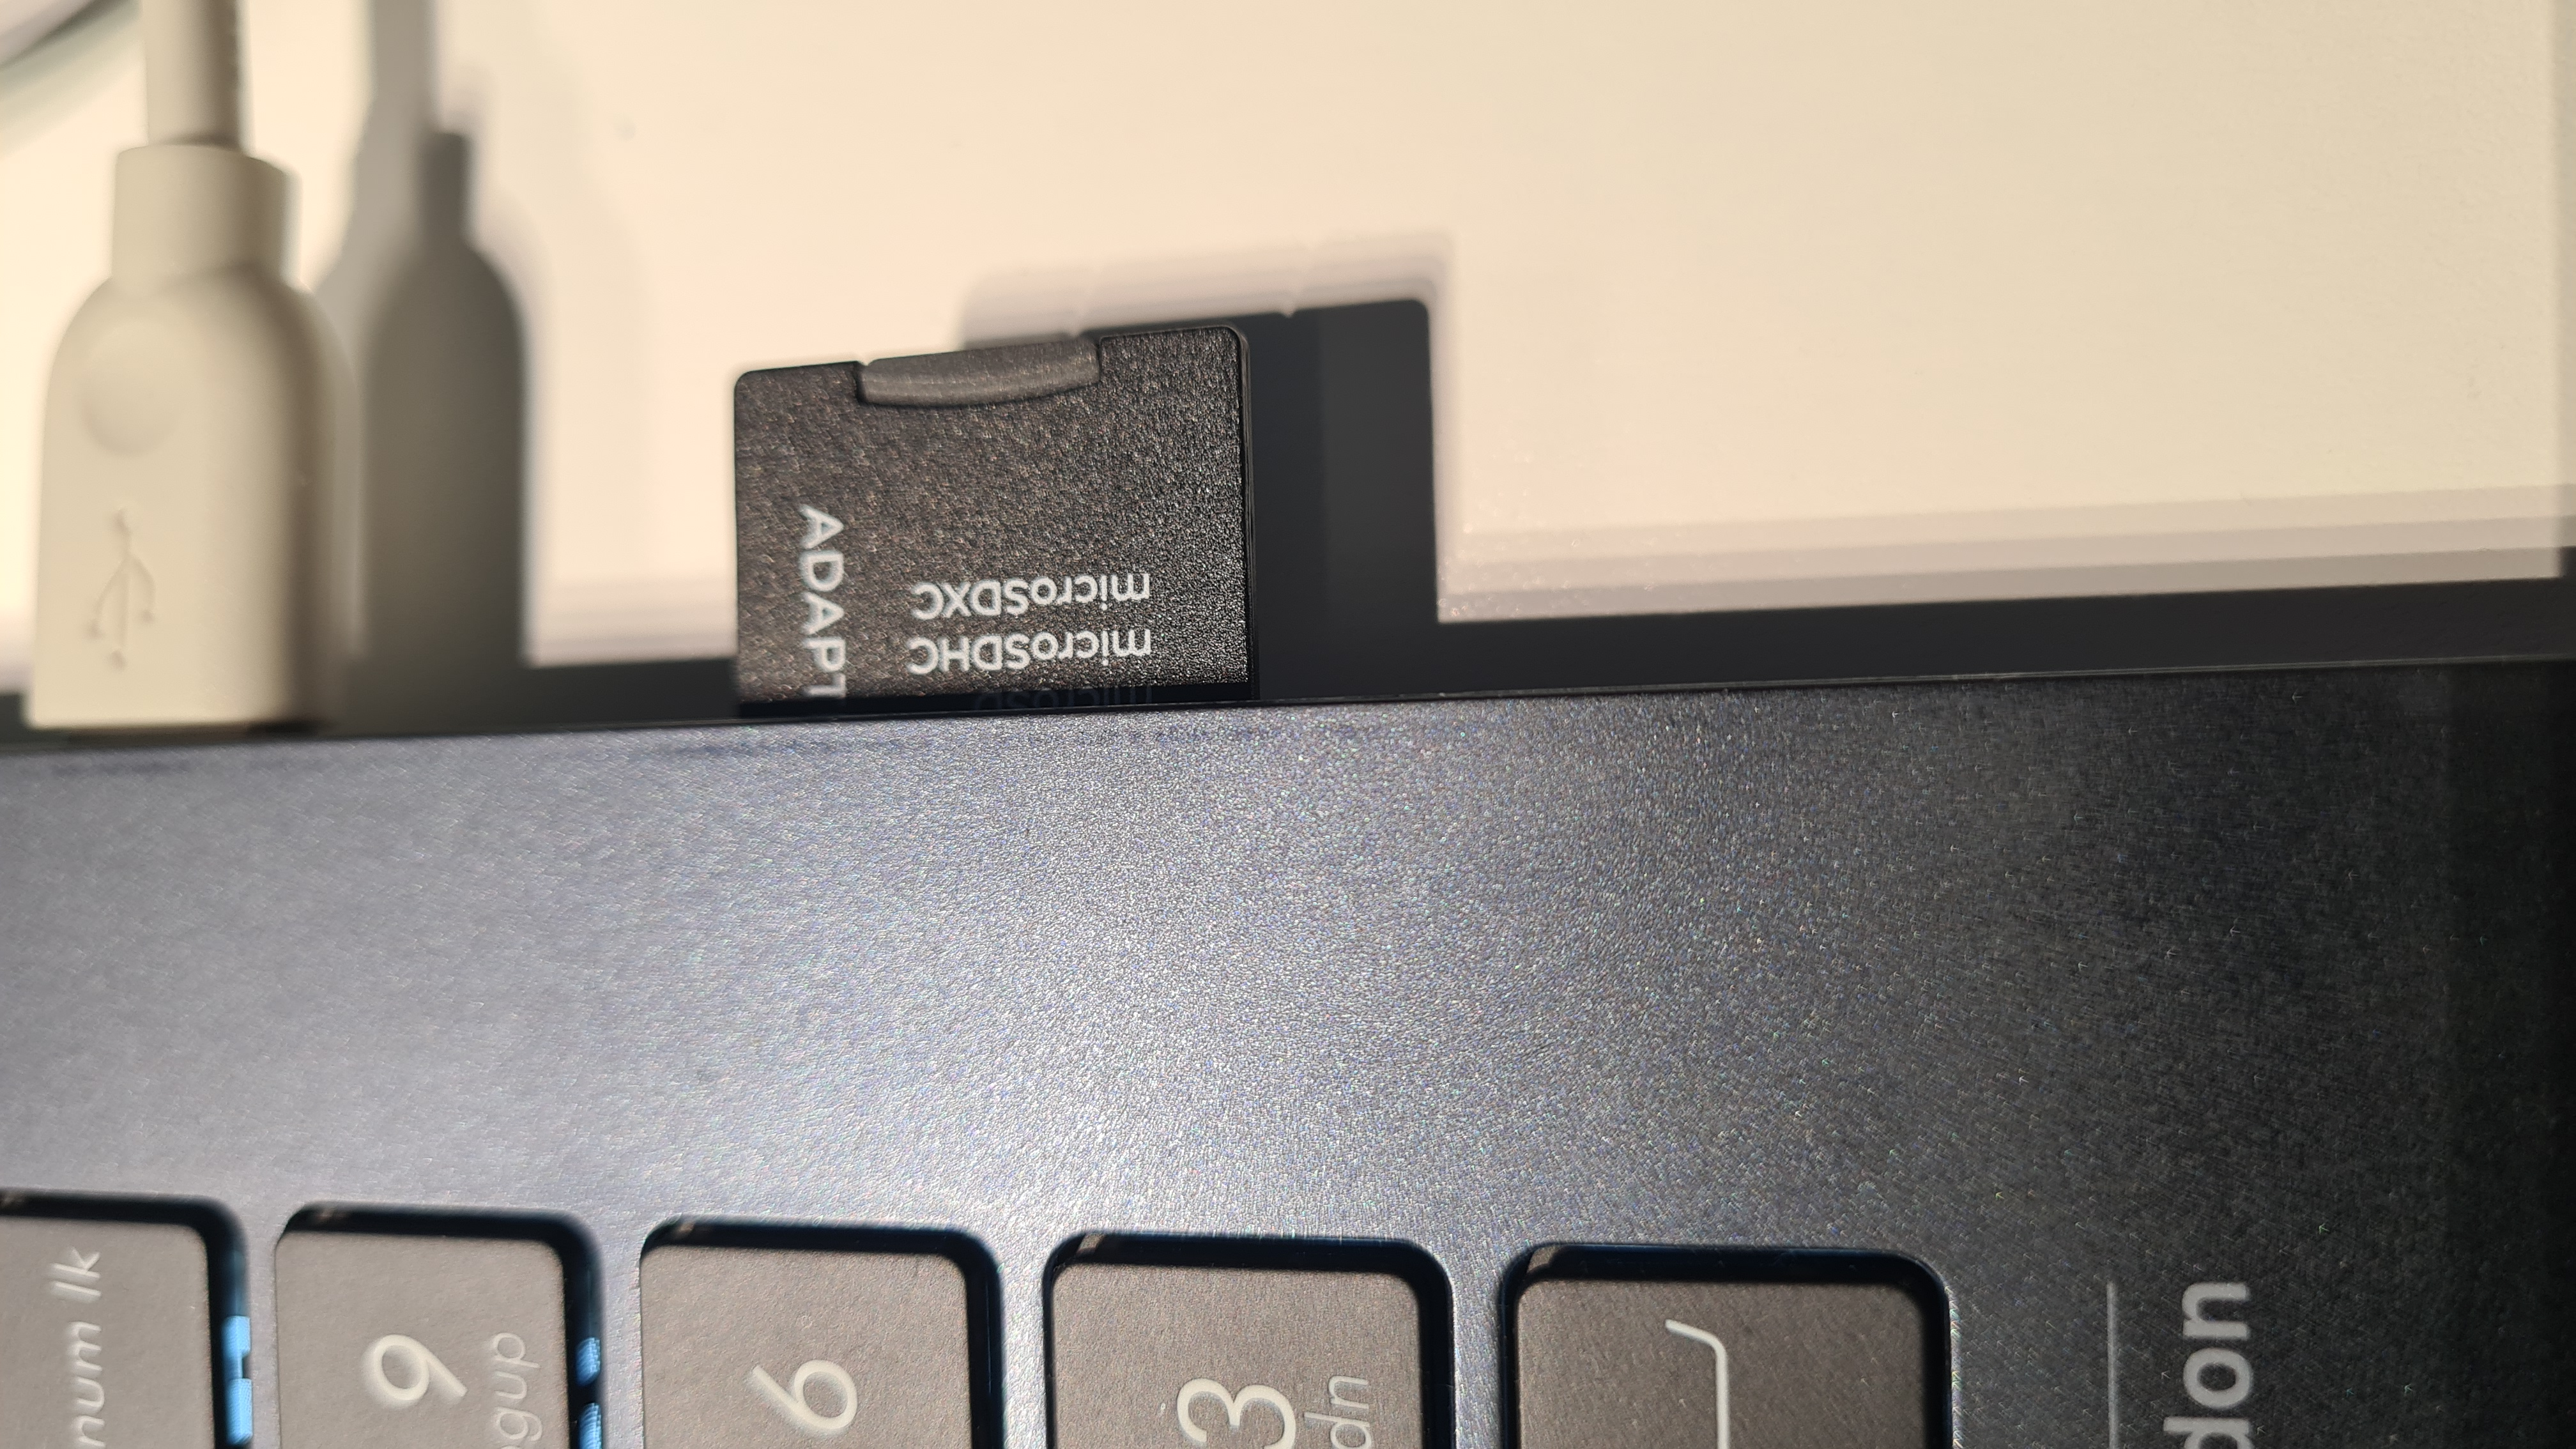
\includegraphics[width=0.6\textwidth]{SDcardPC.jpg}
\caption{Flashing SD card with \code{sdcard.img}}
\label{SDcardPC}
\end{figure}

The files used in this Section resulted from the compilation process seen in Section~\ref{compbuildroot.ch} with the \code{stm32f469\_disco\_sd\_defconfig} configuration. While this is not the board we are working with the CPU architecture is the same.
Firstly, we need to flash our \code{sdcard.img} onto the 4GB SD card provided with the STM32L476G-Eval board, shown in~\ref{SDcardPC}.

\begin{figure}[H]
\centering
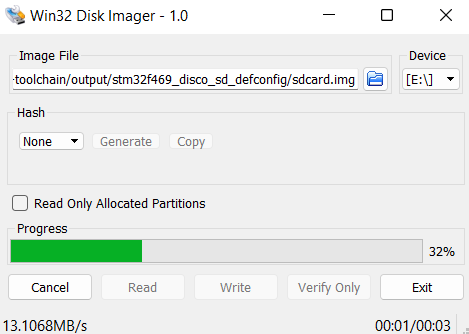
\includegraphics[width=0.6\textwidth]{sdflashing.png}
\caption{Flashing SD card with \code{sdcard.img} using Disk Imager}
\label{sdflashing}
\end{figure}

To achieve this the Disk Imager tool is used, as shown in Figure~\ref{sdflashing}. The process takes less than 3 seconds and is completed successfully. The contents of the SD card are shown in Figure~\ref{SDcontents}.

\begin{figure}[H]
\centering
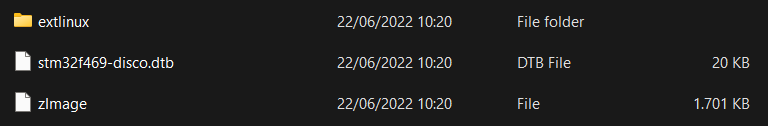
\includegraphics[width=0.6\textwidth]{SDcontents.png}
\caption{Contents of SD card after flashing}
\label{SDcontents}
\end{figure}

Inside the \code{extlinux} folder a single file is found, the \code{extlinux.conf} file. These files are created automatically and are a result of flashing the SD card.

\begin{figure}[H]
\centering
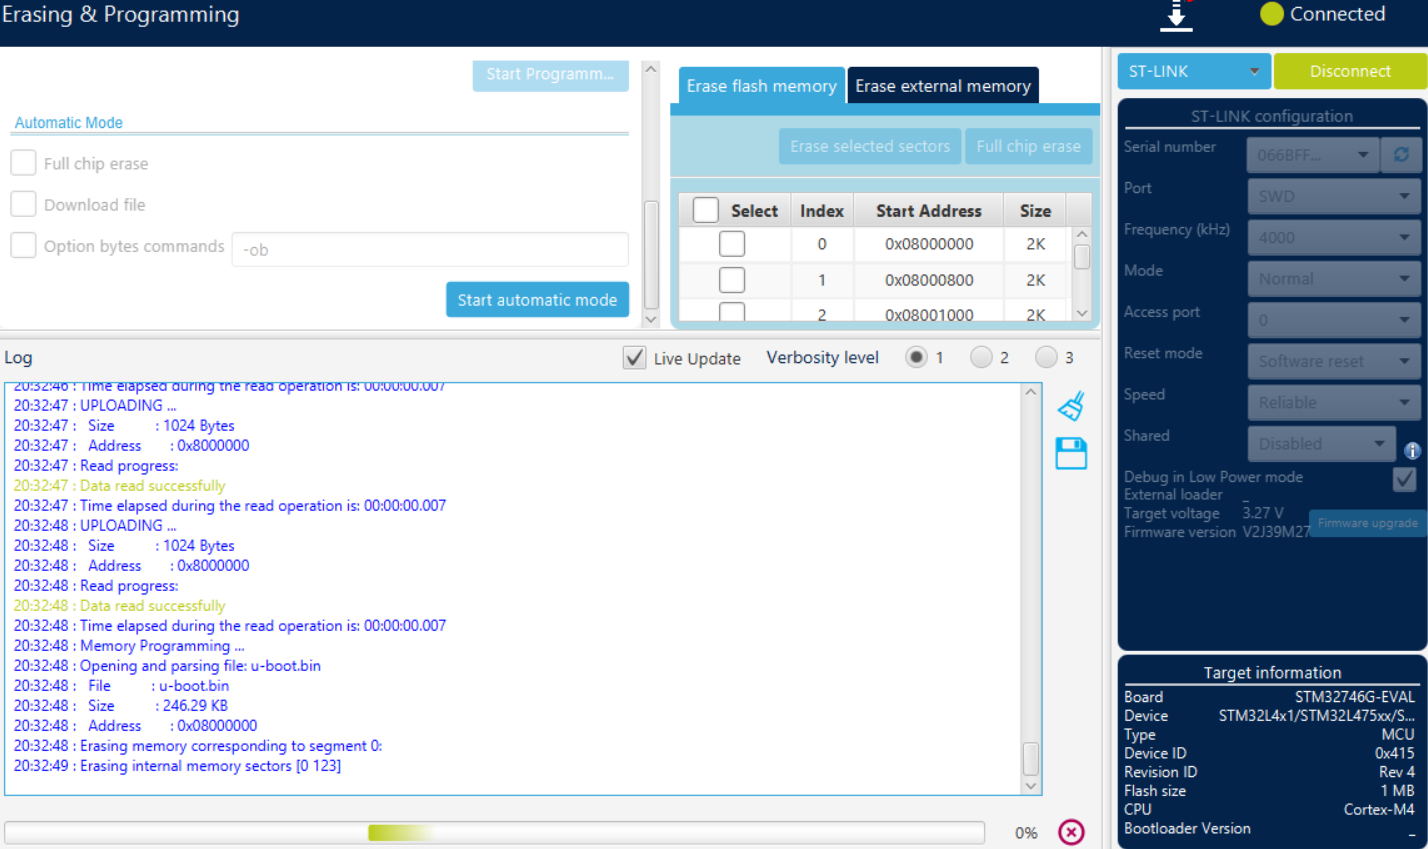
\includegraphics[width=0.9\textwidth]{flashingUboot.png}
\caption{Flashing U-Boot onto internal ROM of STM32L476G-Eval}
\label{flashingUboot}
\end{figure}

Shown in Figure~\ref{flashingUboot}, using the STM32CubeProgrammer tool, we flash \code{u-boot.bin} directly to the MCU. We can observe that the file has a size of \code{246.29 KB} and the starting physical address where it was flashed, namely \code{0x08000000}. In the bottom right, under "Target Information", our board is identified as the one specified earlier.

\begin{figure}[H]
\centering
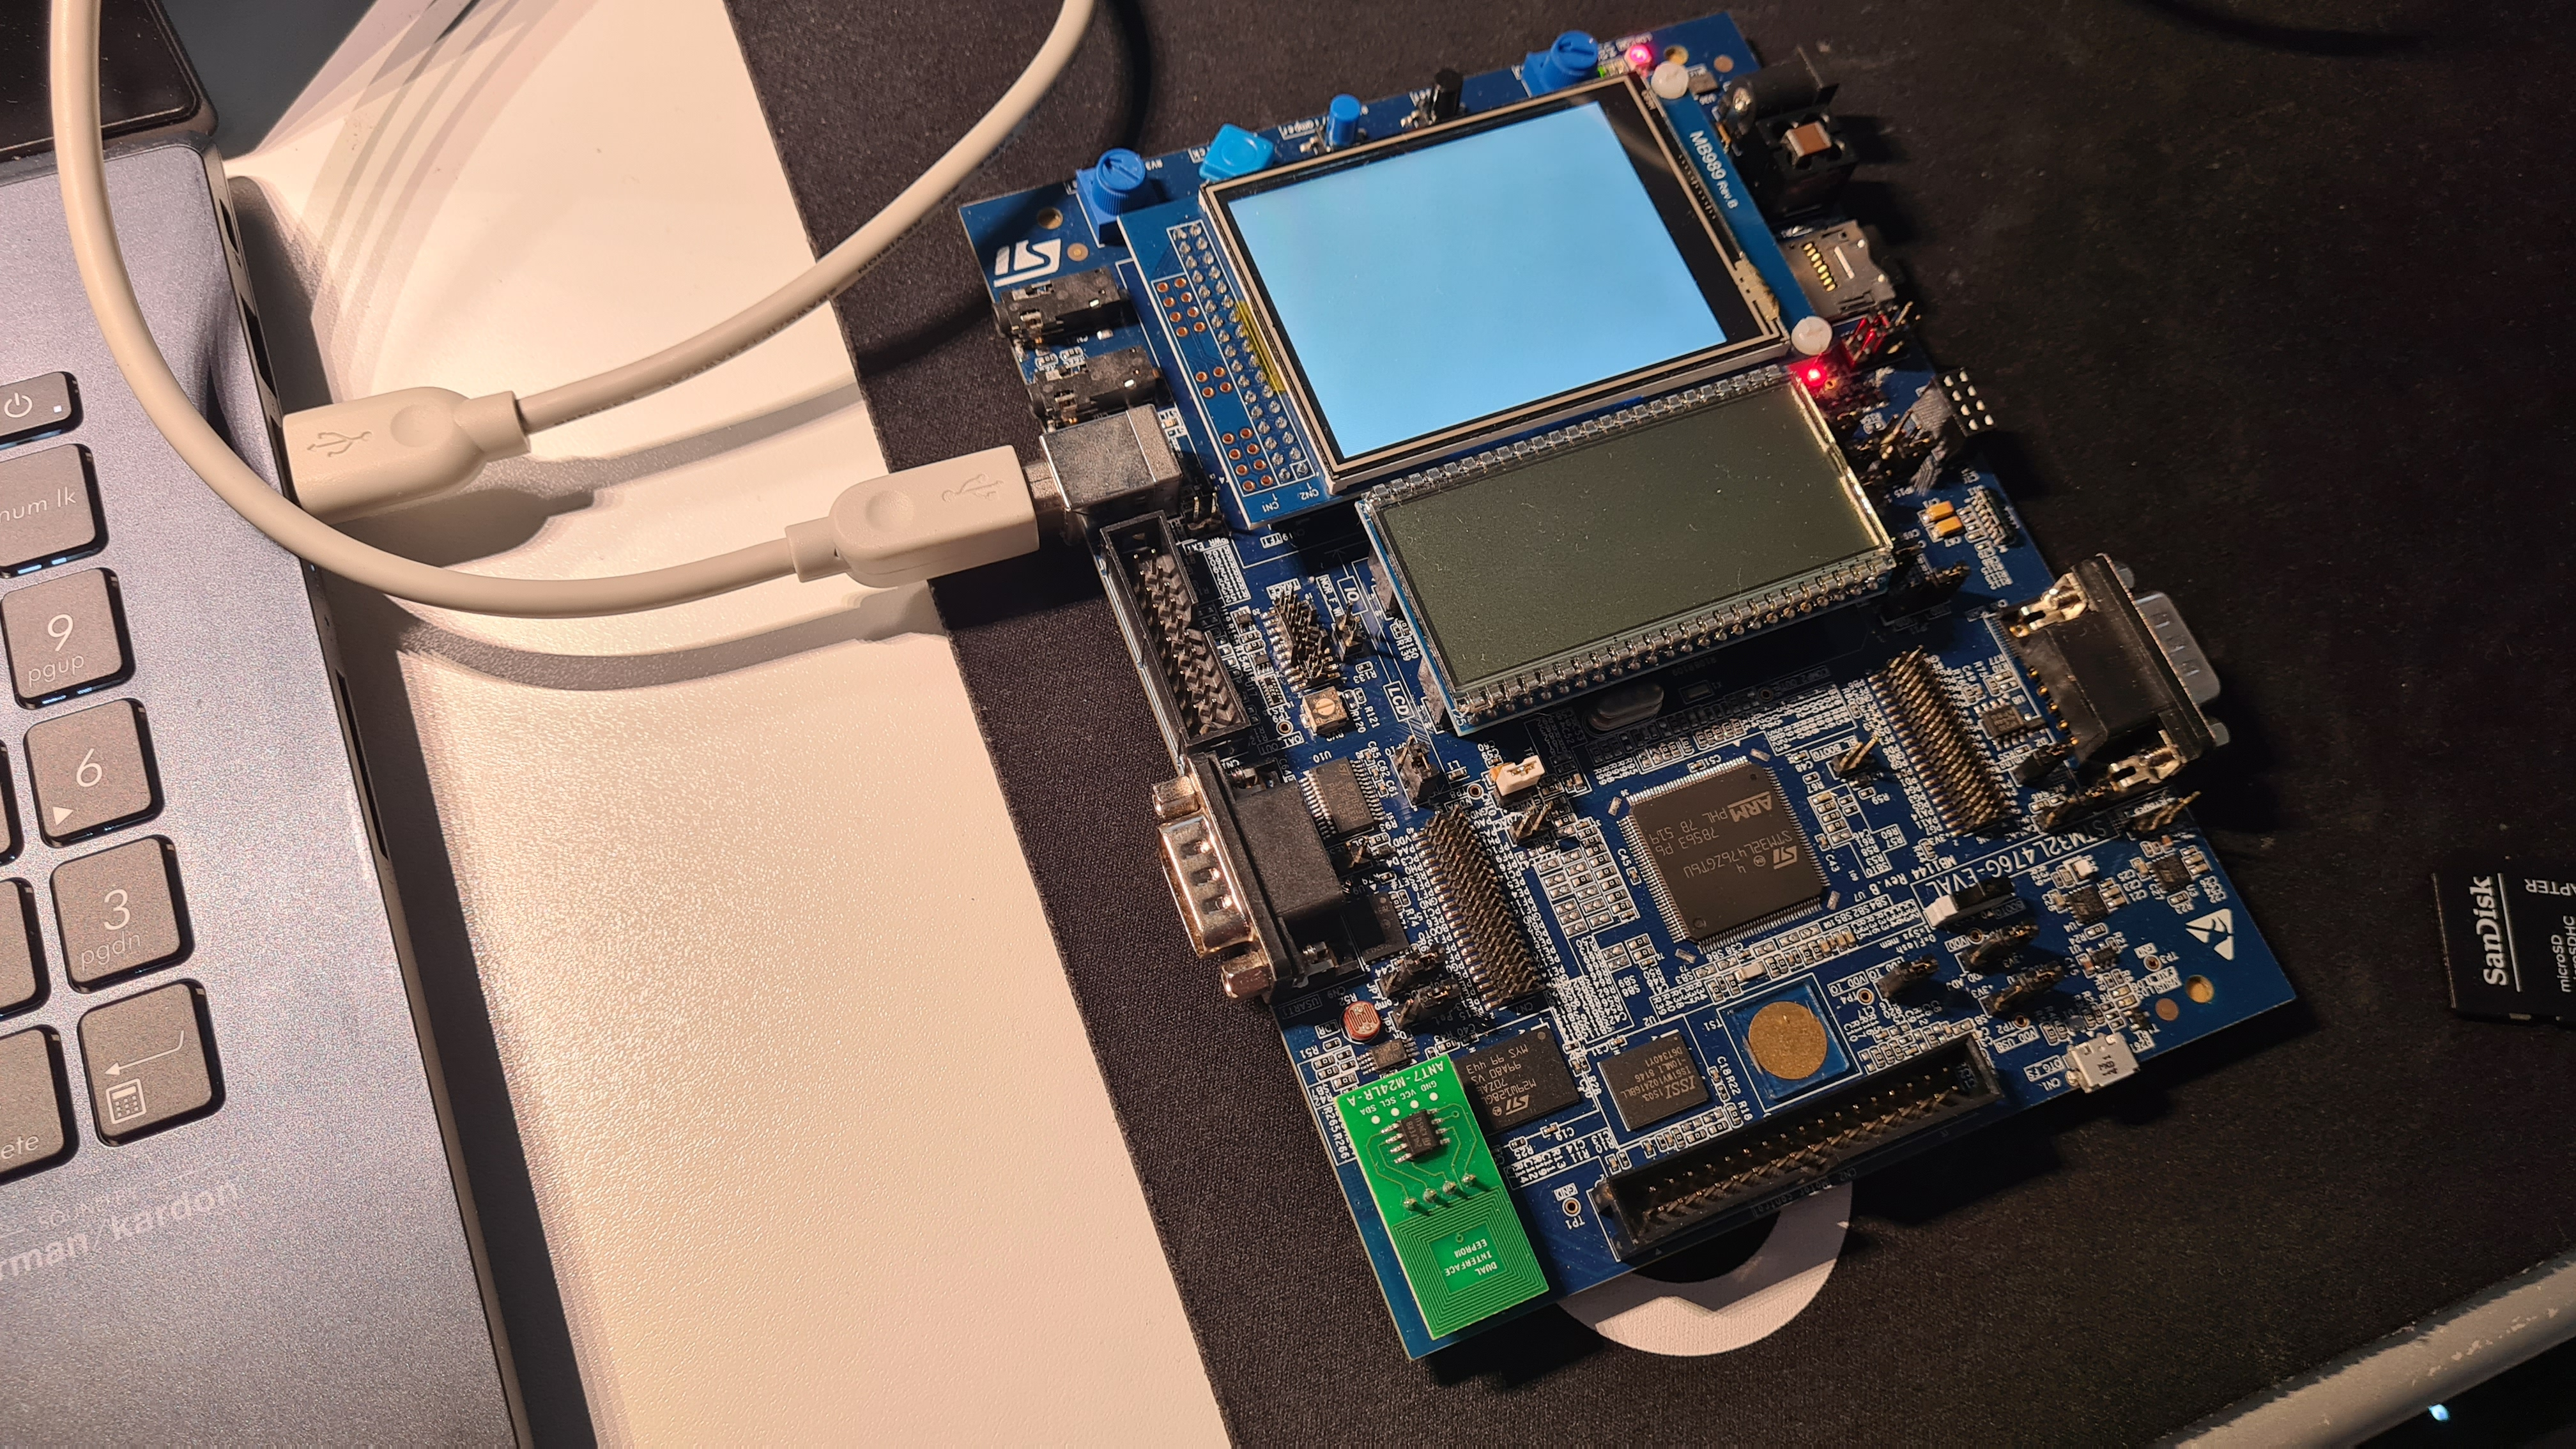
\includegraphics[width=0.8\textwidth]{STLINK.jpg}
\caption{Laptop connected to STM32L476G-Eval through USB Type-B}
\label{usbB}
\end{figure}

In Figure~\ref{usbB} the connection to the board is visible. The ST-Link/V2-1 interface is connected to the PC through a USB Type-B cable, acting as a power source and date exchange simultaneously. While flashing is in progress, the red light in the top right corner flashed rapidly.

\begin{figure}[H]
\centering
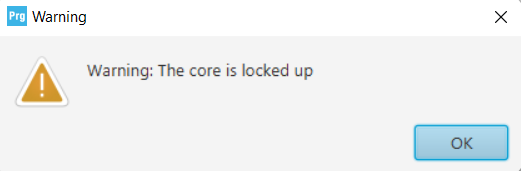
\includegraphics[width=0.5\textwidth]{errorflashinguboot.png}
\caption{Flashing U-Boot: Warning the core is locked up}
\label{errorflashinguboot}
\end{figure}

Upon completion, we get a warning dialog box, seen in Figure~\ref{errorflashinguboot}. The cause of such an error can have various origins, and further investigation is required.

\begin{figure}[H]
\centering
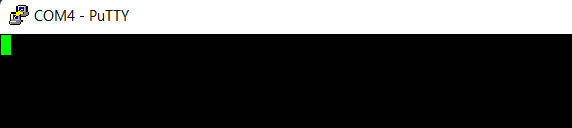
\includegraphics[width=0.7\textwidth]{puttynooutput.png}
\caption{No console output in PuTTY}
\label{puttynooutput}
\end{figure}

Lastly, when connecting to the serial port COM4 using PuTTY, for which we used the same configuration as shown in Figure \ref{puttyjuiceVM}, we can see no output as seen in Figure~\ref{puttynooutput}. A similar output as seen in Figure \ref{buildrootqemu}, was hoped for. Although this was to be expected since the compilation was performed for STM32F469 and not STM32L476, while both employ a Cortex-M4 CPU, this common ground was not enough.
